% E.17 正方形 ABCD 边长 4. E∈BC, F∈CD, BE=CF=x. M=AB 中点. AE 与 BF 交于 P.
% A(0,4), B(4,4), C(4,0), D(0,0). 示例 x=1.5: E=(4, 2.5), F=(2.5, 0). M=(2,4).
% AE: y-4=(2.5-4)/(4-0)·(x-0)= -0.375x → y=4-0.375x
% BF: 从 B(4,4) 到 F(2.5,0). 方向 (-1.5,-4). y-4=4/1.5·(x-4)? 斜率=(0-4)/(2.5-4)= 8/3. y=4+8/3·(x-4)=8x/3-20/3
% 交点 P: 4-0.375x = 8x/3 - 20/3 → 12-1.125x = 8x - 20 → 32 = 9.125x → x=3.507? 重算斜率 BF: (0-4)/(2.5-4)=(-4)/(-1.5)=8/3 ✓
% 4-0.375x=8x/3-20/3 → 乘12: 48-4.5x=32x-80 → 128=36.5x → x≈3.51, y=4-0.375·3.51=2.68
% 嗯不太对; 实际 AE⊥BF, 应在 BF 中点附近. 让我们用更整齐示例: x=2 → E(4,2), F(2,0). AE: y=4-x/2. BF: 从(4,4)到(2,0), 斜率 2, y=2x-4. 交: 4-x/2=2x-4 → 8=2.5x → x=3.2, y=2.4. P=(3.2, 2.4).
\documentclass[tikz,border=4pt]{standalone}
\usepackage{ctex}
\usepackage{amsmath}
\usetikzlibrary{calc}
\begin{document}
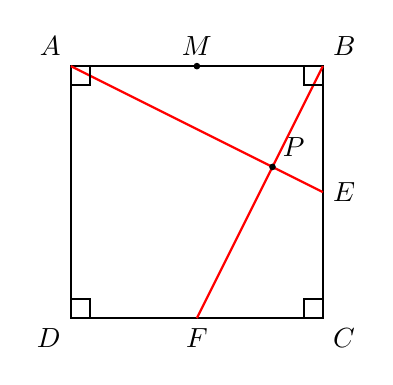
\begin{tikzpicture}[scale=0.8, thick]
  \coordinate (A) at (0,4);
  \coordinate (B) at (4,4);
  \coordinate (C) at (4,0);
  \coordinate (D) at (0,0);
  \coordinate (E) at (4,2);
  \coordinate (F) at (2,0);
  \coordinate (M) at (2,4);
  \coordinate (P) at (3.2, 2.4);

  \draw (A)--(B)--(C)--(D)--cycle;
  \draw[red, thick] (A)--(E);
  \draw[red, thick] (B)--(F);

  \draw ($(A)+(0.3,0)$)--($(A)+(0.3,-0.3)$)--($(A)+(0,-0.3)$);
  \draw ($(B)+(-0.3,0)$)--($(B)+(-0.3,-0.3)$)--($(B)+(0,-0.3)$);
  \draw ($(C)+(-0.3,0)$)--($(C)+(-0.3,0.3)$)--($(C)+(0,0.3)$);
  \draw ($(D)+(0.3,0)$)--($(D)+(0.3,0.3)$)--($(D)+(0,0.3)$);

  \node[above left] at (A) {$A$};
  \node[above right] at (B) {$B$};
  \node[below right] at (C) {$C$};
  \node[below left] at (D) {$D$};
  \node[right] at (E) {$E$};
  \node[below] at (F) {$F$};
  \node[above] at (M) {$M$};
  \node[above right] at (P) {$P$};

  \fill (M) circle (1.5pt);
  \fill (P) circle (1.5pt);
\end{tikzpicture}
\end{document}
